\documentclass[../waterman_intro_comp_bio.tex]{subfiles}
%\usepackage[margin=1in]{geometry}
%\usepackage{amsmath}

\begin{document}
\section{Some Molecular Biology}
    \subsection{Basics}
        \begin{outline}
            \1 Four bases: adenine (A), cytosine (C), quanine (G), and thymine (T)
            \1 Two complementary base pairs: A --- T and G --- C
            \1 DNA is double stranded, RNA is single stranded
                \2 Written from the \(5^{\prime}\) to \(3^{\prime}\) direction, e.g. \(5^{\prime}\) ACCTGAC \(3^{\prime}\)
        \end{outline}

    \subsection{Central Dogma}
        \begin{outline}
            \1 Central dogma of information flow, from Crick (1958)
            
            \begin{displayquote}
                The central dogma states that once `information' has passed into protein it cannot get out again. The transfer of information from nucleic acid to nucleic acid, or from nucleic acid to protein, may be possivle, but transfer from protein to protein, or from protein to nucleic acid, is impossible. Information means here the precise determination of sequence, either of bases in the nucleic acid or of amino acid residues in the protein.
            \end{displayquote}

            \1 DNA \(\rightarrow\) RNA \(\rightarrow\) Protein
                \2 DNA \(\rightarrow\) DNA = replication
                \2 DNA \(\rightarrow\) RNA = transcription
                \2 RNA \(\rightarrow\) Protein = translation
        \end{outline}

    \subsection{The Genetic Code}
        \begin{outline}
            \1 20 amino acids are used to create protein sequences, as determined by Crick.
                \2 Assume sequences are read as blocks of nucleotides, and cannot be less than 3 letters long (since \(4\) and \(4^{2} < 20\) and \(4^3 > 20\)).
                \2 Therefore, if amino acids are encoded by triplets of nucleotides (called \textit{codons}), and the code is comma--free, each reading frame is:
                    \begin{equation*}
                        \underbrace{x_1 x_2 x_3}_{\text{R}_1} ~ \underbrace{x_4 x_5 x_6}_{\text{R}_2} ~\underbrace{x_7 x_8 x_9}_{\text{R}_3} 
                    \end{equation*}
                and not
                    \begin{equation*}
                        x_1 \underbrace{x_2 x_3 x_4}_{\text{R}_1} ~ \underbrace{x_6 x_7 x_8}_{\text{R}_2} ~\underbrace{x_8 x_9 x_{10}}_{\text{R}_3} 
                    \end{equation*}
                etc\ldots
                \2 Each nucleotide needs a reading frame.
                \2 All possible amino acid sequences are possible. However, AAA, TTT, GGG, and CCC are not (since in AAAAAA, for example, there is no obvious reading frame, and four difference places to begin reading AAA). So we're left with \(4^3 - 4\) = 60 combinations.
                \2 As to the others, let XYZ be a codon. to have a comma--free code, XYZXYZ must be read unambiguously. So if XYZ is a codon, YZX and ZXY cannot be. So we're left with \(60 \times \frac{1}{3} = 20 \).
            \1 There are three stop codons, UAA, UAG, and UGA.
            \1 There are many pairs of codons which code for the same amino acid that differ only in the third position, but relatively few which code for the same amino acid while differing in the first or second.
            \1 Assume a sequence UUUUACUGCGGC\ldots
                \2 There are three reading frames in the \(5^{\prime}\) to \(3^{\prime}\) direction and three in the opposite direction from the complementary DNA strand. So a possible of six reading frames for double--stranded DNA.
            \1 Let \textbf{N} \(= \{\text{A, C, G, U}\}\) be the set of nucleic acids, \textbf{C} \(= \{(x_1 x_2 x_3) : x_i \in N\}\), and \textbf{A} be the set of amino acids and termination codon. The genetic code is then just the map \(g : \text{\textbf{C}} \rightarrow \text{\textbf{A}}\) (see Table \ref{gc_table}).
        \begin{table}[]
            \centering
            \begin{tabular}{cccccc}
                \multicolumn{6}{c}{\(2^{\text{nd}}\)}  \\ \hline
                                   & U   & C   & A   & G   &   \\ \hline
                \(1^{\text{st}}\)  &     &     &     &     & \(3^{\text{rd}}\) \\ \hline
                \multirow{4}{*}{U} & Phe & Ser & Tyr & Cos & U \\
                                   & Phe & Ser & Tyr & Cys & C \\
                                   & Leu & Ser & TC  & TC  & A \\
                                   & Leu & Ser & TC  & Trp & G \\ \hline
                \multirow{4}{*}{C} & Leu & Pro & His & Arg & U \\
                                   & Leu & Pro & His & Arg & C \\
                                   & Leu & Pro & Gln & Arg & A \\
                                   & Leu & Pro & Gln & Arg & G \\ \hline
                \multirow{4}{*}{A} & Ile & Thr & Asn & Ser & U \\
                                   & Ile & Thr & Asn & Ser & C \\
                                   & Ile & Thr & Lys & Arg & A \\
                                   & Met & Thr & Lys & Arg & G \\ \hline
                \multirow{4}{*}{G} & Val & Ala & Asp & Gly & U \\
                                   & Val & Ala & Asp & Gly & C \\
                                   & \multicolumn{1}{l}{Val} & \multicolumn{1}{l}{Ala} & \multicolumn{1}{l}{Glu} & \multicolumn{1}{l}{Guy} & \multicolumn{1}{l}{A} \\
                                   & Val & Ala & Glu & Gly & G                    
            \end{tabular}
            \caption{Genetic code. Termination codons indicated by TC.}
            \label{gc_table}
            \end{table}
        \end{outline}

    \subsection{Transfer RNA and Protein Sequences}
        \begin{outline}
            \1 mRNA (messenger RNA) is read to make proteins.
            \1 Amino acids are linked to tRNA (transfer RNA), which then brings them to the mRNA by interacting with codons on the mRNA.
            \1 Since RNA is single stranded, it tends to fold back on itself to form helical regions (Figure \ref{RNA_hairpin}).
                \begin{figure}[h!]
                    \centering
                    
\includegraphics[width=2cm]{ch1/figs/RNA_hairpin.jpg}
                    \caption{Example of RNA folding on itself to create a hairpin.}
                    \label{RNA_hairpin}
                \end{figure}

            \1 tRNA often makes cloverleaf structures, with an \textit{anticodon} at the bottom (Figure \ref{tRNA_cloverleaf}).
                \2 This anticodon is complimentary to the codon on mRNA that the tRNA brings amino acids to.
                \begin{figure}[h!]
                    \centering
                    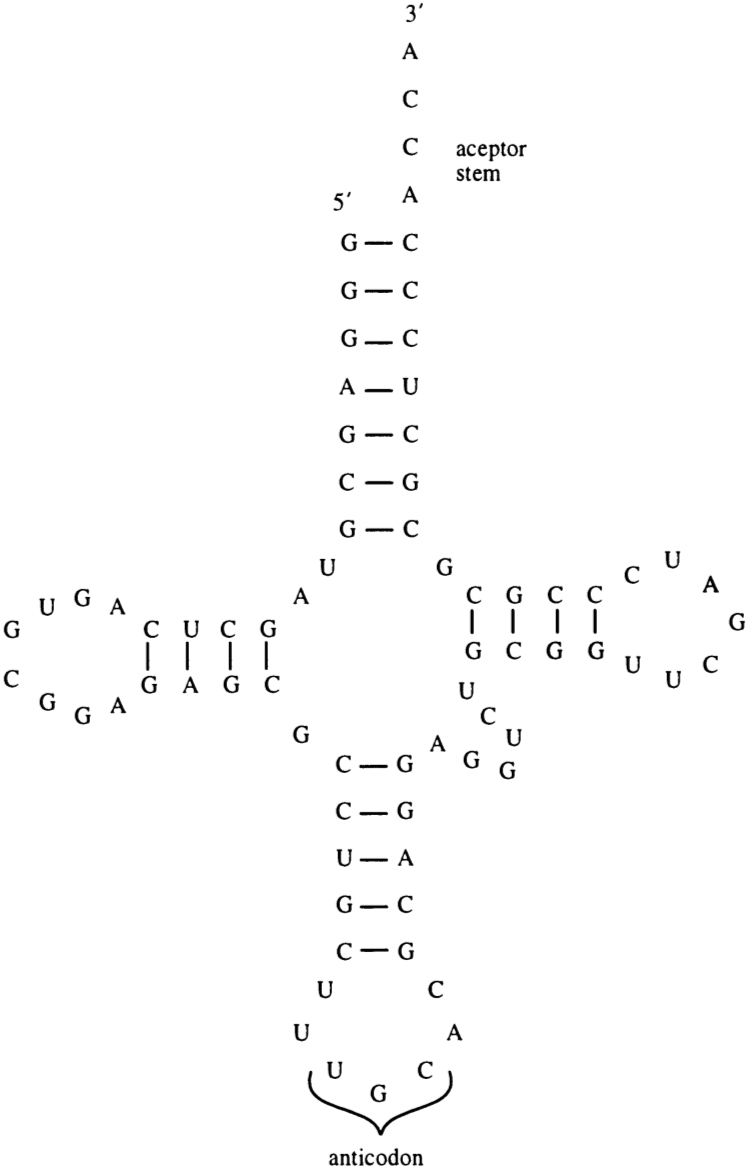
\includegraphics[width=5cm]{ch1/figs/tRNA_cloverleaf.png}
                    \caption{tRNA in cloverleaf structure, showing the anticodon on the bottom leaf.}
                    \label{tRNA_cloverleaf}
                \end{figure}
            \1 mRNA is read at the ribosome, which then uses tRNA to create proteins.
        \end{outline}

    \subsection{Genes Are Not Simple}
        \subsubsection{Start and Stop}
            \begin{outline}
                \1 Three codons which code for ``stop'', one codon which codes for ``begin'' (AUG, coding for Met).
                \1 RNA polymerase, which reads DNA and transcribes mRNA, binds to \textit{promoter sequence} on DNA which sets it up to read down the sequence to the gene.
                    \2 Binds to two sequences: TTGACA (-35) and TATAAT (-10), with numbers indicating nucleotide distance from start codon
                    \2 Note: there is no position ``0'' when numbering sequences.
            \end{outline}

        \subsubsection{Gene Expression Control}
            \begin{outline}
                \1 Expression can be controlled at one of two points: DNA \(\rightarrow\) RNA or RNA \(\rightarrow\) Protein.
                \1 Example of RNA \(\rightarrow\) DNA control:
                    \2 A molecule called a \textit{repressor} binds to DNA stopping the expression of a protein which processes a particular molecule.
                    \2 When the particular protein is present, it binds to the repressor and prevents it from binding to DNA.
                    \2 When all of the molecule has been used in whatever process it's used in, the repressor is then free to bind to the DNA and stop transcription of its processor protein.
            \end{outline}

        \subsubsection{Split Genes}
            \begin{outline}
                \1 DNA encoding proteins are interrupted by noncoding DNA which disappears in mRNA.
                    \2 For example, a gene \textit{E} is expected to be one contiguous region, but are split by noncoding regions \(I_1\) and \(I_2\) to form a noncontinuous gene \(E_1\), \(E_2\), and \(E_3\)
                    \2 The split gene sections (\(E\)) are called \textit{exons} and the noncoding regions (\(I\)) are called \textit{introns}.
                    \2 Introns are separated out during transcription, and the exons become a contiguous gene on mRNA.
                \1 The vast majority of DNA is non--encoding -- in humans, only 5\% is used in protein coding
            \end{outline}

        \subsubsection{Jumping Genes}
            \begin{outline}
                \1 There exist in both prokaryotic and eukaryotic genomes genes which move from place to place in the genome.
                    \2 Called \textit{transposable elements}.
                    \2 Carry genes required for transposition, and are called ``jumping genes''.
                \1 These can propagate themselves, creating identical segments of DNA
                \1 Function is not known, some speculate they're ``selfish'' genes which exist only to propagate themselves, much like miniature organisms (fucking rad)
            \end{outline}

        \subsection{Biological Chemistry}
            \begin{outline}
                \1 Skipping most of this, as it's just chemistry.
            \end{outline}

            \subsubsection{DNA}
                \begin{outline}
                    \1 DNA is composed of four different subunits, or \textit{nucleotides}.
                        \2 \textit{Adenine}, \textit{guanine}, \textit{thymine}, and \textit{cytosine}. Adenine and guanine have a purine as a base, and thymine and cytosine have pyrimidines as a base.
                        \2 Each nucleotide is composed to a phosphate group and a base attached to a five--membered, oxygen containing ring (Fig.~\ref{ch1:nucleotide}). In DNA, this sugar is 2--deoxyribose
                            \begin{figure}
                                \centering
                                \includegraphics[width=1.5in]{ch1/figs/nucleotide.jpeg}
                                \label{ch1:nucleotide}
                                \caption{Nucleotide template.}
                            \end{figure}

                    \1 A single strand of DNA is formed by phosphate bonds connecting the sugars of the nucleotides (Fig~\ref{ch1:phosphate}).
                        \begin{figure}
                            \centering
                            \includegraphics[width=2in]{ch1/figs/phosphate_bonds.jpeg}
                            \label{ch1:phosphate}
                            \caption{Single strand of DNA showing the nucleotides connected by phosphate bonds.}
                        \end{figure}

                \end{outline}

            \subsubsection{RNA}
                \begin{outline}
                    \1 Ribonucleic acid (RNA) is quite similar to DNA, except its sugar is ribose, not 2--deoxyribose.
                    \1 The nucleotide thymine is replaced with uracil.
                \end{outline}

\end{document}
